\chapter{Corrosion et protection}\label{ch:b2:corrosion}

Déposons une goutte d'eau salée sur un morceau d'acier propre. Au bout d'un jour, le métal est
piqué au centre de la goutte, tandis que la rouille s'est formée en anneau près de son
bord, là où se dissout le dioxygène de l'air. Le fer se dissout là où il y a
le moins de dioxygène, et le dioxygène est réduit là où il y en a le plus~: la goutte
est une pile que personne n'a construite, court-circuitée par le métal lui-même. Ce
chapitre lit la corrosion sur les \omterm{def:b2:current-potential-curves:ie-curve}{courbes intensité--potentiel}, explique pourquoi une
tôle galvanisée rayée ne rouille pas alors qu'une boîte de conserve en fer-blanc rayée rouille, et
conçoit la protection d'un pipeline enterré.

\begin{recall}
Le volume de première année~: diagrammes E--pH des métaux et leurs domaines d'immunité,
corrosion et \omterm{def:b2:corrosion:passivation}{passivation} («~savoir si une couche protège est une question de cinétique~»).
\Cref{ch:b2:current-potential-curves}~: \omterm{def:b2:current-potential-curves:ie-curve}{courbes intensité--potentiel}, \omterm{def:b2:current-potential-curves:limiting-current}{courants
limites}. \Cref{ch:b2:batteries-electrolysis}~: le \omterm{def:b2:batteries-electrolysis:mixed-potential}{potentiel mixte}. Le volume
scolaire~: corrosion, rouille, galvanisation.
\end{recall}

\begin{omfigure}
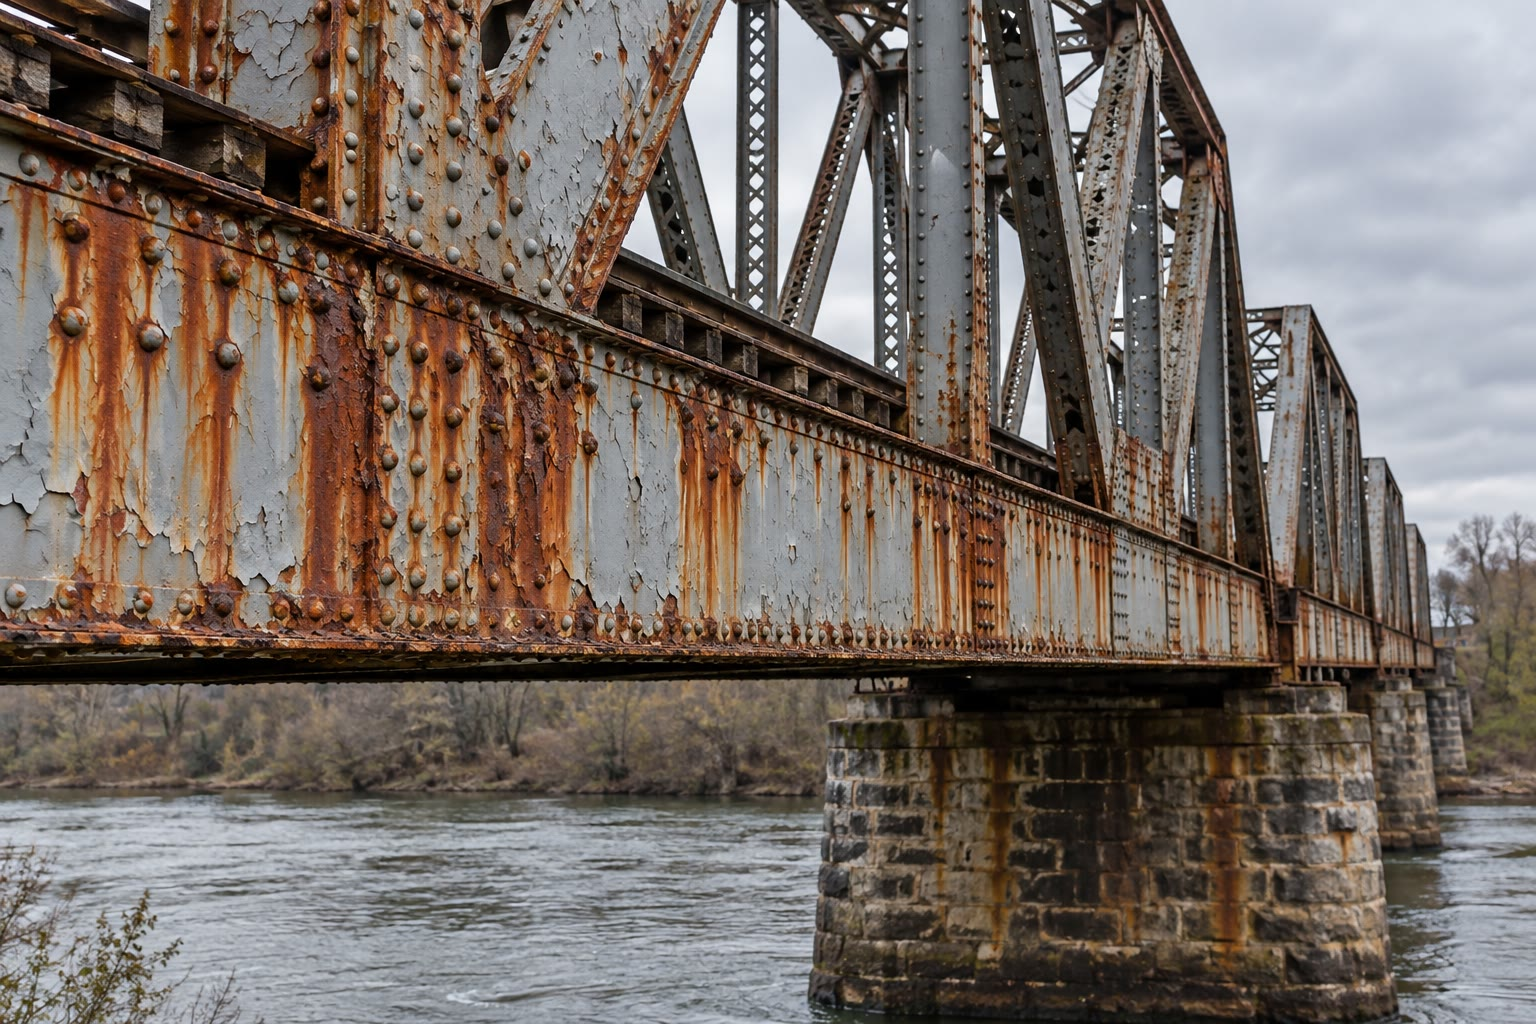
\includegraphics[width=0.62\linewidth]{images/book3/ai/b2-12-rusty-bridge.jpg}

{\small Un vieux pont ferroviaire riveté. Des coulures de rouille descendent des rivets
et des joints, là où l'eau et le dioxygène séjournent le plus longtemps et où la peinture cède
en premier.}
\end{omfigure}

\section{La corrosion humide, une pile en court-circuit}

Dans une eau contenant du dioxygène dissous, le fer est oxydé, \ce{Fe -> Fe^2+ + 2e-},
et les électrons sont captés sur le même morceau de métal par la réduction du
dioxygène, \ce{O2 + 2H2O + 4e- -> 4OH-} (en milieu acide, aussi par \ce{2H+ + 2e- -> H2}). Les
ions fer(II) et les ions hydroxyde se rencontrent dans l'eau, et une oxydation ultérieure par
l'air transforme leur précipité en rouille, un oxyde de fer(III) hydraté.

\begin{definition}[Corrosion uniforme]\label{def:b2:corrosion:uniform}
La \emph{corrosion uniforme}\index{corrosion uniforme} est la corrosion d'un métal
dont l'oxydation et la réduction de l'oxydant ont lieu en des sites répartis
uniformément sur sa surface. Le \emph{potentiel de corrosion}\index{potentiel de corrosion}
est le \omterm{def:b2:batteries-electrolysis:mixed-potential}{potentiel mixte} que prend alors le métal, et le
\emph{courant de corrosion}\index{courant de corrosion} est le \omterm{def:b2:current-potential-curves:ie-curve}{courant anodique}
d'oxydation du métal à ce potentiel.
\end{definition}

\begin{omfigure}
\begin{tikzpicture}
\begin{axis}[omie, width=0.82\linewidth, height=5.6cm, xmin=-1.1, xmax=0.5,
  ymin=-1.6, ymax=1.6, xlabel={$E$}, ylabel={$i$}, clip=true, clip mode=individual,
  axis y line=left]
\addplot[omanodic] table[x=E, y=i] {figdata/out/bachelor-2-ie-curves-i-Fe.dat};
\addplot[omcathodic] table[x=E, y=i] {figdata/out/bachelor-2-ie-curves-i-O2.dat};
\addplot[omcathodic, densely dashed] table[x=E, y=i, y expr=-\thisrow{i}] {figdata/out/bachelor-2-ie-curves-i-O2.dat};
\draw[densely dotted] (axis cs:-0.394,-1.0) -- (axis cs:-0.394,1.0);
\fill (axis cs:-0.394,1.0) circle (1.4pt);
\node[font=\scriptsize, anchor=south east] at (axis cs:-0.40,1.02) {$i_{\text{corr}}$};
\node[font=\scriptsize, anchor=north west] at (axis cs:-0.39,-0.03) {$E_{\text{corr}}$};
\node[font=\scriptsize, omThm, anchor=west] at (axis cs:-0.35,1.4) {\ce{Fe} $\to$ \ce{Fe^2+}};
\node[font=\scriptsize, omDef, anchor=north west] at (axis cs:-0.75,-1.05) {\ce{O2} $\to$ \ce{OH-}, palier de diffusion};
\end{axis}
\end{tikzpicture}

{\small Le diagramme d'Evans du fer dans une eau neutre aérée (courbes modèles). La
courbe cathodique du dioxygène est aussi tracée réfléchie vers le haut (en tirets)~: le
\omterm{def:b2:corrosion:uniform}{potentiel de corrosion} se situe là où elle rencontre la courbe anodique du fer. Comme la
réduction du dioxygène y a atteint son palier de diffusion, le \omterm{def:b2:corrosion:uniform}{courant de
corrosion} est égal au \omterm{def:b2:current-potential-curves:limiting-current}{courant limite} du dioxygène~: agiter ou aérer l'eau
fait corroder le fer plus vite.}
\end{omfigure}

\begin{proposition}[Vitesse de corrosion]\label{prop:b2:corrosion:rate}
Un métal de masse molaire $M$ et de masse volumique $\rho$, oxydé avec $n$ électrons par
atome sous une densité de \omterm{def:b2:corrosion:uniform}{courant de corrosion} $j_{\text{corr}}$ (courant par unité de surface),
perd par unité de surface et de temps la masse $j_{\text{corr}}M/(nF)$, soit une
épaisseur
\[
  \frac{de}{dt} = \frac{j_{\text{corr}}\,M}{nF\rho} .
\]
\end{proposition}

\begin{proof}
D'après la \cref{prop:b2:current-potential-curves:current-rate}, la densité de \omterm{def:b2:current-potential-curves:ie-curve}{courant
anodique} $j_{\text{corr}}$ oxyde $j_{\text{corr}}/(nF)$ moles de métal par unité de surface et de
temps~; multiplier par $M$ pour la masse et diviser par $\rho$ pour l'épaisseur.
\end{proof}

\begin{example}[Le fer à \qty{10}{\micro A/cm^2}]\label{ex:b2:corrosion:rate}
Avec $j = \qty{0.10}{A/m^2}$, $M = \qty{55.845}{g/mol}$, $n = 2$, $\rho =
\qty{7.87}{g/cm^3}$~: $de/dt = 0.10 \times 55.845/(2 \times 96\,485 \times 7.87
\times 10^6) = \qty{3.7e-12}{m/s}$, soit \qty{0.12}{mm} par an.
% ledger: aw:Fe, rho:Fe, const:F
\end{example}

\section{La corrosion différentielle}

\begin{definition}[Corrosion différentielle]\label{def:b2:corrosion:differential}
La \emph{corrosion différentielle}\index{corrosion differentielle@corrosion différentielle} est une corrosion dans
laquelle les sites anodiques et cathodiques sont séparés, le métal étant
oxydé préférentiellement aux sites anodiques. On parle de \emph{corrosion
galvanique}\index{corrosion galvanique} lorsque deux métaux différents en contact électrique
baignent dans le même électrolyte, et d'\emph{aération
différentielle}\index{aeration differentielle@aération différentielle} lorsqu'un même métal est exposé à des eaux de
teneurs en dioxygène différentes.
\end{definition}

\begin{proposition}[Deux métaux en contact]\label{prop:b2:corrosion:galvanic}
Lorsque deux métaux en contact électrique plongent dans la même eau aérée, ils
prennent un même \omterm{def:b2:batteries-electrolysis:mixed-potential}{potentiel mixte}. Le métal dont le \omterm{def:b2:corrosion:uniform}{potentiel de corrosion} est le plus bas
devient l'anode et se corrode plus vite que seul~; l'autre devient une cathode,
sur laquelle le dioxygène est réduit, et il est protégé.
\end{proposition}

\begin{proof}
Reliés par un conducteur de résistance négligeable, les deux métaux sont au
même potentiel, où la somme de tous les \omterm{def:b2:current-potential-curves:ie-curve}{courants anodiques} est égale à l'opposé de la somme de
tous les \omterm{def:b2:current-potential-curves:ie-curve}{courants cathodiques}. La courbe anodique du métal le moins noble monte la première~;
au potentiel commun, elle porte presque tout le \omterm{def:b2:current-potential-curves:ie-curve}{courant anodique}, et le
dioxygène est réduit sur toute la surface mouillée, y compris celle du métal le plus noble,
dont le \omterm{def:b2:current-potential-curves:ie-curve}{courant anodique} propre y est négligeable.
\end{proof}

\begin{omfigure}
\begin{tikzpicture}
\begin{axis}[omie, width=0.82\linewidth, height=5.6cm, xmin=-1.1, xmax=0.5,
  ymin=-2.4, ymax=2.4, xlabel={$E$}, ylabel={$i$}, clip=true, clip mode=individual,
  axis y line=left]
\addplot[omanodic] table[x=E, y=i] {figdata/out/bachelor-2-ie-curves-i-Fe.dat};
\addplot[omanodic, densely dashed] table[x=E, y=i] {figdata/out/bachelor-2-ie-curves-j-Zn.dat};
\addplot[omcathodic] table[x=E, y=i] {figdata/out/bachelor-2-ie-curves-i-O2.dat};
\addplot[omcathodic, densely dashed] table[x=E, y=i] {figdata/out/bachelor-2-ie-curves-j-O2Cu.dat};
\fill (axis cs:-0.394,1.0) circle (1.4pt);
\fill (axis cs:-0.794,1.0) circle (1.4pt);
\fill (axis cs:-0.366,2.0) circle (1.4pt);
\draw[densely dotted] (axis cs:-1.1,1.0) -- (axis cs:-0.394,1.0);
\draw[densely dotted] (axis cs:-1.1,2.0) -- (axis cs:-0.366,2.0);
\node[font=\scriptsize, anchor=south west] at (axis cs:-0.38,0.95) {fer seul};
\node[font=\scriptsize, anchor=west] at (axis cs:-0.35,2.0) {fer + cuivre};
\node[font=\scriptsize, anchor=south east] at (axis cs:-0.80,1.05) {fer + zinc};
\node[font=\scriptsize, omThm, anchor=north west] at (axis cs:-0.98,0.75) {zinc};
\node[font=\scriptsize, omThm, anchor=north west] at (axis cs:-0.55,0.75) {fer};
\node[font=\scriptsize, omDef, anchor=north east] at (axis cs:0.45,-2.05) {\ce{O2} sur fer + cuivre};
\node[font=\scriptsize, omDef, anchor=north east] at (axis cs:0.45,-1.05) {\ce{O2} sur fer};
\end{axis}
\end{tikzpicture}

{\small Le fer couplé à d'autres métaux (courbes modèles). Avec le zinc, le potentiel
commun s'abaisse jusqu'à ce que le zinc porte le \omterm{def:b2:current-potential-curves:ie-curve}{courant anodique}~: le fer est protégé,
le zinc se corrode. Avec le cuivre, la surface cathodique offerte au dioxygène double~: le
\omterm{def:b2:corrosion:uniform}{courant de corrosion} du fer double aussi.}
\end{omfigure}

\begin{proposition}[Aération différentielle]\label{prop:b2:corrosion:aeration}
Sur un métal exposé à des eaux de teneurs en dioxygène différentes, la zone la moins aérée
est anodique et se corrode~; la zone la mieux aérée est cathodique.
\end{proposition}

\begin{proof}
Là où la teneur en dioxygène est plus élevée, le couple \ce{O2}/\ce{OH-} a un potentiel de
Nernst plus élevé et un \omterm{def:b2:current-potential-curves:limiting-current}{courant limite} plus grand~: la courbe cathodique est plus haute
et s'étend plus loin. Le métal, conducteur unique, se fixe à un seul potentiel~;
le fort \omterm{def:b2:current-potential-curves:ie-curve}{courant cathodique} disponible dans la zone aérée doit être compensé par un
\omterm{def:b2:current-potential-curves:ie-curve}{courant anodique}, qui circule là où le métal peut être oxydé avec peu de
concurrence de la réduction du dioxygène, c'est-à-dire dans la zone mal aérée. L'oxydation
s'y concentre.
\end{proof}

\begin{omfigure}
\begin{tikzpicture}[font=\small, >={Stealth}]
  \fill[black!20] (-4.2,-0.7) rectangle (4.2,0);
  \node[font=\scriptsize] at (3.7,-0.35) {acier};
  \fill[omDef!15] (-3.4,0) .. controls (-2.9,2.2) and (2.9,2.2) .. (3.4,0) -- cycle;
  \draw[thick, omDef] (-3.4,0) .. controls (-2.9,2.2) and (2.9,2.2) .. (3.4,0);
  \fill[omProp!80] (-0.7,0) arc[start angle=180, end angle=360, x radius=0.7, y radius=0.22] -- cycle;
  \fill[brown!70!black] (-1.9,0.12) ellipse (0.45 and 0.11);
  \fill[brown!70!black] (1.9,0.12) ellipse (0.45 and 0.11);
  \node[font=\scriptsize, align=center] at (0,2.45) {\ce{O2} de l'air};
  \draw[->, thick, omDef] (-1.0,2.25) -- (-2.6,0.35);
  \draw[->, thick, omDef] (1.0,2.25) -- (2.6,0.35);
  \node[font=\scriptsize, align=center, anchor=east] at (-4.1,1.3) {cathode\\ (bord)};
  \draw[->, thin] (-4.1,1.3) -- (-3.05,0.12);
  \node[font=\scriptsize, align=center, anchor=west] at (4.1,1.3) {anneau de rouille};
  \draw[->, thin] (4.1,1.3) -- (2.3,0.2);
  \draw[->, omThm] (-0.4,-0.3) .. controls (-1.2,-0.5) and (-2.4,-0.5) .. (-3.0,-0.15);
  \draw[->, omThm] (0.4,-0.3) .. controls (1.2,-0.5) and (2.4,-0.5) .. (3.0,-0.15);
  \draw[->, thin] (0,-1.05) -- (0,-0.25);
  \node[font=\scriptsize, anchor=north] at (0,-1.05) {anode (centre)~: \ce{Fe -> Fe^2+ + 2e-}};
  \node[font=\scriptsize, omThm, anchor=north] at (0,-1.45) {les électrons circulent dans l'acier jusqu'au bord};
  \node[font=\scriptsize, anchor=north] at (0,-1.85) {cathode (bord)~: \ce{O2 + 2H2O + 4e- -> 4OH-}};
\end{tikzpicture}

{\small La goutte d'Evans sur l'acier, schéma. Le dioxygène se dissout à la surface et
atteint le métal surtout près du bord mince de la goutte, qui devient la
cathode~; le centre, privé de dioxygène, est l'anode et se creuse de piqûres. Les
ions fer(II) et les ions hydroxyde se rencontrent entre les deux, où la rouille
précipite en anneau.}
\end{omfigure}

Le même mécanisme attaque les interstices, les parties d'une structure situées sous un dépôt
ou un joint, et un pieu d'acier dans la mer juste au-dessous de la ligne de flottaison, où
l'eau est moins aérée qu'en surface.

\begin{method}[Diagnostiquer une corrosion]\label{met:b2:corrosion:diagnose}
\begin{enumerate}
  \item Recenser les métaux en contact et l'électrolyte~; vérifier qu'ils sont
        reliés électriquement.
  \item Pour deux métaux, celui dont le \omterm{def:b2:corrosion:uniform}{potentiel de corrosion} est le plus bas (en général
        celui dont le potentiel standard est le plus bas) est l'anode.
  \item Pour un seul métal, repérer les zones les moins aérées (interstices, dessous des dépôts,
        fond d'une goutte)~: elles sont anodiques.
  \item La vitesse est fixée par la réaction cathodique (apport de dioxygène, surface de la cathode)~:
        une petite anode sur une grande cathode se corrode vite.
\end{enumerate}
\end{method}

\section{La passivation}

\begin{definition}[Passivation]\label{def:b2:corrosion:passivation}
La \emph{passivation}\index{passivation} est la forte diminution de la vitesse de
corrosion d'un métal lorsqu'il se recouvre d'une couche mince, compacte et adhérente de son
oxyde, le \emph{film passif}\index{film passif}, qui le sépare de la
solution. Un métal dans cet état est dit passif.
\end{definition}

\begin{proposition}[Le palier de passivité]\label{prop:b2:corrosion:passivity}
La courbe anodique d'un métal passivable monte à partir de son \omterm{def:b2:corrosion:uniform}{potentiel de corrosion},
atteint un pic, puis retombe à un faible courant passif presque constant sur un
domaine de potentiels, avant de remonter aux potentiels élevés (domaine
transpassif~: oxydation du film ou de l'eau). L'état passif peut se rompre
localement, par exemple sous l'action des ions chlorure, ce qui donne des piqûres.
\end{proposition}

\begin{proof}[Argument]
Aux faibles \omterm{def:b2:current-potential-curves:overpotential}{surtensions}, le métal nu se dissout de plus en plus vite. Au-delà d'un
seuil, l'oxyde devient stable à la surface (le domaine de \omterm{def:b2:corrosion:passivation}{passivation} du
diagramme E--pH) et forme un film que les ions ne traversent que lentement~: le
courant s'effondre jusqu'à ce faible flux. Aux potentiels élevés, le film lui-même est
oxydé en espèces solubles, ou l'eau est oxydée à sa surface. Les ions chlorure, petits
et fortement complexants, peuvent dissoudre le film en ses points faibles, où le métal
mis à nu se corrode alors comme une petite anode face à une immense cathode passive. L'allure
de la courbe est ici celle d'un modèle.
\end{proof}

\begin{omfigure}
\begin{tikzpicture}
\begin{axis}[omie, width=0.82\linewidth, height=5.4cm, xmin=-0.7, xmax=1.5,
  ymin=-0.1, ymax=1.3, xlabel={$E$}, ylabel={$i$}, clip=true, clip mode=individual,
  axis y line=left]
\addplot[omanodic] table[x=E, y=i] {figdata/out/bachelor-2-ie-curves-k.dat};
\node[font=\scriptsize, anchor=south] at (axis cs:-0.33,1.0) {actif};
\node[font=\scriptsize, anchor=south] at (axis cs:0.5,0.06) {palier de passivité};
\node[font=\scriptsize, anchor=east] at (axis cs:1.25,0.9) {transpassif};
\draw[<-, thin] (axis cs:-0.2,0.55) -- (axis cs:0.15,0.7) node[right, font=\scriptsize] {formation du film};
\end{axis}
\end{tikzpicture}

{\small Courbe anodique d'un métal passivable (modèle). Le courant, élevé tant que
le métal nu se dissout, s'effondre quand le \omterm{def:b2:corrosion:passivation}{film passif} se forme, et reste
faible sur un large domaine de potentiels avant la remontée transpassive.}
\end{omfigure}

Les aciers inoxydables contiennent assez de chrome pour former un \omterm{def:b2:corrosion:passivation}{film passif} d'oxyde de chrome
qui se reforme de lui-même à l'air~; l'aluminium est protégé par son film d'alumine, qui
rend un métal situé bien au-dessous de l'hydrogène dans la classification utilisable pour les cadres de fenêtres et
les canettes de boisson. Le cuivre verdit à l'air libre, la patine étant une couche de
sels basiques de cuivre qui ralentit l'attaque ultérieure.

\begin{omfigure}
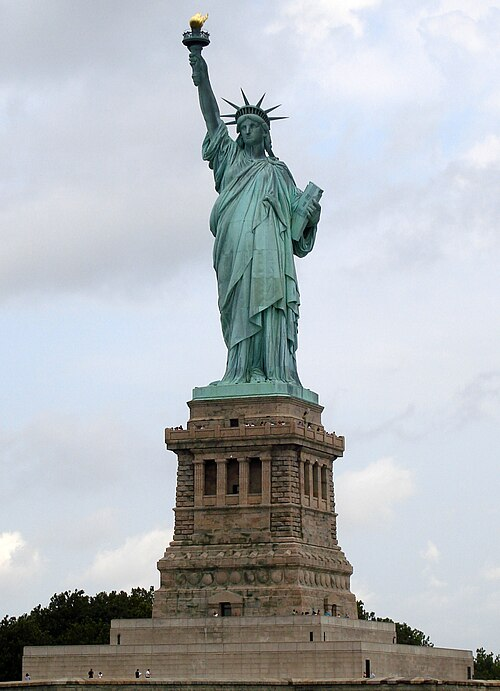
\includegraphics[width=0.32\linewidth]{images/book3/liberty.jpg}

{\small Une statue de cuivre plus que centenaire~: sa peau de fine tôle de cuivre
a verdi, recouverte d'une patine de sels basiques de cuivre qui protège le
métal sous-jacent. (Photographie~: Elcobbola, domaine public, Wikimedia Commons.)}
\end{omfigure}

\section{La protection}

On combat la corrosion en séparant le métal de l'eau et du dioxygène (peinture,
plastique, émail, ou couche d'un autre métal), en modifiant le milieu
(élimination du dioxygène, ajout d'inhibiteurs qui s'adsorbent sur le métal), ou en déplaçant le
potentiel du métal dans son domaine d'immunité.

\begin{definition}[Protection cathodique]\label{def:b2:corrosion:protection}
La \emph{protection cathodique}\index{protection cathodique} abaisse le potentiel d'une
structure métallique jusqu'à l'arrêt de son oxydation, en en faisant la cathode d'une pile.
La pile peut être formée avec une \emph{anode sacrificielle}\index{anode sacrificielle},
un métal moins noble (zinc, magnésium, alliages d'aluminium) relié à la
structure et consommé à sa place, ou être entraînée par un générateur, dans la
\emph{protection par courant imposé}\index{protection par courant impose@protection par courant imposé},
l'anode étant alors une électrode inerte enterrée à proximité.
\end{definition}

\begin{proposition}[Durée de vie d'une anode sacrificielle]\label{prop:b2:corrosion:anode-life}
Une \omterm{def:b2:corrosion:protection}{anode sacrificielle} de masse $m$ et de masse molaire $M$, oxydée avec $n$ électrons
et un rendement $\eta$ (fraction du métal qui produit un courant utile,
le reste se corrodant de lui-même), débite un courant $I$ pendant une durée
\[
  t = \frac{\eta\,m\,nF}{M I} .
\]
\end{proposition}

\begin{proof}
La charge utile vaut $\eta\,(m/M)\,nF$~; il reste à diviser par le courant.
\end{proof}

\begin{omfigure}
\begin{tikzpicture}[font=\small, >={Stealth}]
  \fill[brown!20] (-4.2,-2.4) rectangle (4.2,0);
  \draw[thick] (-4.2,0) -- (4.2,0);
  \node[font=\scriptsize, anchor=south west] at (-4.2,0) {sol};
  \fill[black!40] (-3.5,-1.6) rectangle (3.5,-1.2);
  \node[font=\scriptsize, white] at (0,-1.4) {conduite en acier (cathode)};
  % sacrificial anode
  \fill[black!65] (-3.2,-2.3) rectangle (-2.2,-1.95);
  \node[font=\scriptsize, anchor=north] at (-2.7,-2.3) {anode en Mg};
  \draw[thick] (-2.7,-1.95) -- (-2.7,-1.6);
  \draw[->, omProp, thick] (-2.2,-2.12) -- (-1.4,-1.7);
  \node[font=\scriptsize, omProp, anchor=west] at (-1.9,-2.2) {courant dans le sol};
  % impressed current
  \draw[thick, rounded corners] (1.8,0.4) rectangle (3.2,1.2);
  \node[font=\scriptsize] at (2.5,0.8) {redresseur};
  \fill[black!65] (3.4,-2.3) rectangle (3.9,-1.8);
  \node[font=\scriptsize, anchor=north] at (3.65,-2.3) {anode inerte};
  \draw[thick] (3.2,0.8) -- (3.65,0.8) -- (3.65,-1.8);
  \draw[thick] (1.8,0.8) -- (1.2,0.8) -- (1.2,-1.2);
  \node[font=\scriptsize, anchor=south] at (3.65,0.85) {$+$};
  \node[font=\scriptsize, anchor=south] at (1.2,0.85) {$-$};
  \node[font=\scriptsize, align=center] at (-2.7,0.8) {anode sacrificielle};
  \node[font=\scriptsize, align=center] at (2.5,1.55) {courant imposé};
\end{tikzpicture}

{\small \omterm{def:b2:corrosion:protection}{Protection cathodique} d'une conduite enterrée, schéma. À gauche~: une anode
en magnésium, reliée à la conduite, se corrode à sa place. À droite~: un redresseur fait circuler
un courant d'une anode inerte à travers le sol jusqu'à la conduite.}
\end{omfigure}

\begin{omfigure}
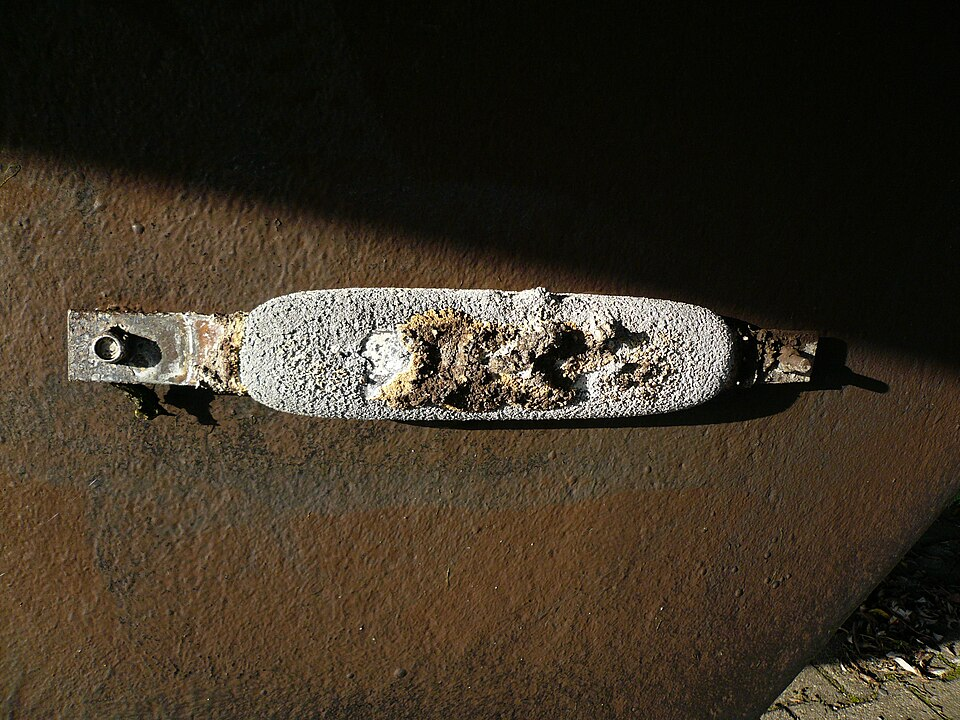
\includegraphics[width=0.5\linewidth]{images/book3/sacrificial-anode.jpg}

{\small Une \omterm{def:b2:corrosion:protection}{anode sacrificielle} en zinc boulonnée sur la coque en acier d'un bateau, après une
saison dans l'eau~: le zinc est rongé, l'acier qui l'entoure est intact.
(Photographie~: Zwergelstern, CC BY-SA 3.0, Wikimedia Commons.)}
\end{omfigure}

\begin{omfigure}
\begin{tikzpicture}[font=\small, >={Stealth}, scale=1.35]
  \begin{scope}
    \fill[black!25] (0,0) rectangle (4,0.6);
    \fill[gray!55] (0,0.6) rectangle (1.7,0.8); \fill[gray!55] (2.3,0.6) rectangle (4,0.8);
    \fill[omDef!15] (0.8,0.8) .. controls (1.3,1.3) and (2.7,1.3) .. (3.2,0.8) -- (2.3,0.8) -- (2.3,0.6) -- (1.7,0.6) -- (1.7,0.8) -- cycle;
    \node[font=\scriptsize] at (2,-0.3) {acier galvanisé (couche de zinc)};
    \node[font=\scriptsize, align=center] at (2,1.6) {le zinc se corrode,\\ l'acier est protégé};
    \draw[->, omThm] (1.4,0.85) -- (1.8,0.65);
  \end{scope}
  \begin{scope}[xshift=5.5cm]
    \fill[black!25] (0,0) rectangle (4,0.6);
    \fill[gray!25] (0,0.6) rectangle (1.7,0.8); \fill[gray!25] (2.3,0.6) rectangle (4,0.8);
    \fill[omDef!15] (0.8,0.8) .. controls (1.3,1.3) and (2.7,1.3) .. (3.2,0.8) -- (2.3,0.8) -- (2.3,0.6) -- (1.7,0.6) -- (1.7,0.8) -- cycle;
    \fill[omProp] (1.75,0.6) rectangle (2.25,0.45);
    \node[font=\scriptsize] at (2,-0.3) {acier étamé (couche d'étain)};
    \node[font=\scriptsize, align=center] at (2,1.6) {l'acier se corrode dans la rayure,\\ vite (petite anode)};
  \end{scope}
\end{tikzpicture}

{\small Une rayure à travers un revêtement métallique, schéma. Le zinc, moins noble que
le fer, devient l'anode et protège l'acier mis à nu, quelle que soit la taille de
la rayure. L'étain, plus noble que le fer, devient une grande cathode autour d'une petite
anode d'acier, qui se corrode plus vite que ne le ferait l'acier nu.}
\end{omfigure}

\begin{method}[Choisir une protection]\label{met:b2:corrosion:choose-protection}
\begin{enumerate}
  \item Éviter les couples galvaniques~: isoler les métaux différents, ou donner au moins
        noble la plus grande surface.
  \item Revêtir~: un revêtement barrière (peinture, étain) ne protège que tant qu'il est intact~; un
        revêtement sacrificiel (zinc) protège même rayé.
  \item Pour une structure dans le sol ou dans l'eau de mer, ajouter une \omterm{def:b2:corrosion:protection}{protection cathodique}~:
        \omterm{def:b2:corrosion:protection}{anodes sacrificielles} pour les faibles courants ou les eaux conductrices,
        courant imposé pour les longues structures ou les sols résistants.
  \item Ne pas surprotéger~: un potentiel trop bas réduit l'eau en dihydrogène sur
        la structure, ce qui décolle les revêtements et peut fragiliser les aciers à haute
        résistance.
\end{enumerate}
\end{method}

\section{Exercices}

\begin{exercise}[$\star$]\label{exo:b2:corrosion:1}
Du zinc se corrode uniformément sous une densité de courant de \qty{2.0}{\micro A/cm^2}.
Calculer sa perte d'épaisseur par an ($\rho = \qty{7.13}{g/cm^3}$).
\end{exercise}

\begin{exercise}[$\star$]\label{exo:b2:corrosion:2}
Des boulons en acier maintiennent des feuilles de cuivre sur un toit. Quel métal se corrode~? Même question
pour des clous en zinc dans des tôles d'acier.
\end{exercise}

\begin{exercise}[$\star$]\label{exo:b2:corrosion:3}
Deux plaques d'acier sont assemblées par un boulon et laissées dans l'eau de mer. Où
la corrosion se concentre-t-elle, et pourquoi~?
\end{exercise}

\begin{exercise}[$\star$]\label{exo:b2:corrosion:4}
Un seau galvanisé et une boîte en fer-blanc sont tous deux rayés jusqu'à l'acier. Lequel
rouille au niveau de la rayure~?
\end{exercise}

\begin{exercise}[$\star\star$]\label{exo:b2:corrosion:5}
Sur le diagramme d'Evans du fer dans l'eau aérée, expliquer ce que deviennent le
potentiel et le \omterm{def:b2:corrosion:uniform}{courant de corrosion} lorsqu'on agite l'eau, puis lorsqu'on
en élimine le dioxygène.
\end{exercise}

\begin{exercise}[$\star\star$]\label{exo:b2:corrosion:6}
Une anode de zinc de \qty{5.0}{kg} protège une coque de bateau avec un courant de
\qty{0.10}{A} et un rendement de 90~\% (données de l'exercice). Combien de temps
dure-t-elle~?
\end{exercise}

\begin{exercise}[$\star\star$]\label{exo:b2:corrosion:7}
Calculer la charge, en ampères-heures par kilogramme, fournie par des anodes de zinc, de magnésium
et d'aluminium avec un rendement de 100~\%, ainsi que les potentiels standard de
leurs couples à partir des $\Delta_f G^\circ$ (\ce{Zn^2+} $-147.06$, \ce{Mg^2+} $-454.8$,
\ce{Al^3+} $-485$ \unit{kJ/mol}). Pourquoi préfère-t-on le magnésium dans les sols secs~?
\end{exercise}

\begin{exercise}[$\star\star$]\label{exo:b2:corrosion:8}
Une conduite enterrée exige un courant de protection de \qty{2.0}{A}. Le lit d'anode
inerte présente une résistance de \qty{4.0}{\ohm} par rapport au sol et la cellule exige
\qty{1.5}{V} supplémentaires (données de l'exercice). Calculer la tension du redresseur et
l'énergie électrique par an.
\end{exercise}

\begin{exercise}[$\star\star$]\label{exo:b2:corrosion:9}
Un pieu d'acier se dresse dans la mer. Expliquer pourquoi il se corrode le plus un peu au-dessous de
la ligne de flottaison, et non à la ligne de flottaison elle-même.
\end{exercise}

\begin{exercise}[$\star\star\star$]\label{exo:b2:corrosion:10}
Expliquer, à l'aide de la courbe de passivité, pourquoi l'acier inoxydable résiste à l'eau aérée mais
peut se piquer dans l'eau de mer, et pourquoi une piqûre, une fois amorcée, se creuse plutôt
qu'elle ne s'élargit.
\end{exercise}

\begin{exercise}[$\star\star\star$]\label{exo:b2:corrosion:11}
Un raccord en cuivre est vissé sur une conduite en acier transportant de l'eau aérée. La densité
de \omterm{def:b2:current-potential-curves:limiting-current}{courant limite} du dioxygène vaut \qty{5}{\micro A/cm^2} sur toute surface mouillée~; le
cuivre offre \qty{20}{cm^2} et l'acier proche du raccord \qty{2}{cm^2}
(données de l'exercice). Estimer le \omterm{def:b2:corrosion:uniform}{courant de corrosion} de l'acier et sa perte
d'épaisseur par an près du raccord.
\end{exercise}

\begin{exercise}[$\star\star\star$]\label{exo:b2:corrosion:12}
À l'aide du diagramme E--pH du fer et des courbes de l'eau, expliquer pourquoi le
potentiel d'une structure en acier protégée doit être maintenu au-dessous d'environ
\qty{-0.6}{V}, mais pas bien au-dessous de \qty{-1}{V}, dans une eau neutre.
\end{exercise}

\section{Problème~: protéger un pipeline}

\begin{problem}[{Problème du week-end --- la corrosion d'une conduite en acier nu dans un sol
humide, le choix d'un métal sacrificiel, le magnésium nécessaire pour vingt ans,
et la solution du courant imposé}]
\label{pb:b2:corrosion:1}
Un pipeline en acier de \qty{10.0}{km} de long et de \qty{0.30}{m} de diamètre est enterré dans
un sol humide. Données~: fer $M = \qty{55.845}{g/mol}$, $\rho = \qty{7.87}{g/cm^3}$~;
magnésium $M = \qty{24.305}{g/mol}$~; $\Delta_f G^\circ$ (\unit{kJ/mol})~: \ce{Fe^2+}
$-78.90$, \ce{Zn^2+} $-147.06$, \ce{Mg^2+} $-454.8$, \ce{Al^3+} $-485$. Données de
l'exercice~: densité de \omterm{def:b2:corrosion:uniform}{courant de corrosion} de l'acier nu dans ce sol \qty{10}{\micro
A/cm^2}~; densité de courant de dimensionnement pour la protection de l'acier nu
\qty{20}{mA/m^2}~; le revêtement laisse 1.0~\% de la surface à nu~; anodes de magnésium
de \qty{15}{kg}, rendement 50~\%~; résistance du lit d'anode pour le courant imposé
\qty{5.0}{\ohm}.
% ledger: aw:Fe, rho:Fe, aw:Mg, dfg:Fe2+_ao, dfg:Zn2+_ao, dfg:Mg2+_ao, dfg:Al3+_ao, const:F

\medskip
\noindent\textbf{Partie I --- La conduite nue.}
\begin{enumerate}
  \item Écrire les réactions anodique et cathodique sur la conduite.
  \item Pourquoi le \omterm{def:b2:corrosion:uniform}{courant de corrosion} est-il fixé par l'apport de dioxygène~?
  \item Calculer la masse de fer perdue par mètre carré et par an.
  \item Calculer la perte d'épaisseur de paroi par an.
  \item Combien de temps la conduite nue mettrait-elle à perdre la moitié d'une paroi de \qty{8}{mm}~?
  \item Pourquoi la conduite réelle cède-t-elle plus tôt, en quelques points~?
\end{enumerate}

\medskip
\noindent\textbf{Partie II --- Le métal de l'anode.}
\begin{enumerate}[resume]
  \item Calculer les potentiels standard des couples du fer, du zinc, du magnésium
        et de l'aluminium.
  \item Quels métaux peuvent protéger le fer comme \omterm{def:b2:corrosion:protection}{anodes sacrificielles}~?
  \item Pourquoi l'aluminium est-il peu utilisé dans les sols~?
  \item Pourquoi préfère-t-on le magnésium au zinc dans un sol de forte résistivité~?
  \item Calculer la masse de magnésium consommée par ampère et par an.
\end{enumerate}

\medskip
\noindent\textbf{Partie III --- Le dimensionnement.}
\begin{enumerate}[resume]
  \item Calculer la surface extérieure de la conduite.
  \item Calculer la surface laissée à nu par le revêtement.
  \item Calculer le courant de protection.
  \item Calculer la charge nécessaire pour vingt ans.
  \item Calculer la masse de magnésium nécessaire.
  \item Combien d'anodes faut-il~?
  \item Pourquoi les répartit-on le long de la conduite plutôt que de les enterrer en un
        seul point~?
\end{enumerate}

\medskip
\noindent\textbf{Partie IV --- Le courant imposé.}
\begin{enumerate}[resume]
  \item Décrire la solution du courant imposé.
  \item Estimer la tension du redresseur à partir de la résistance du lit d'anode,
        en ajoutant \qty{1.5}{V} pour les électrodes.
  \item Calculer l'énergie électrique consommée par an.
  \item Que se passe-t-il si la conduite est surprotégée~?
  \item Au-dessous de quel potentiel le fer est-il immunisé dans une eau neutre, en prenant une
        concentration en fer(II) de \qty{1e-6}{mol/L}~?
  \item Donner la masse d'anodes de magnésium nécessaire pour vingt ans.
\end{enumerate}
\end{problem}
